\begin{figure*}[p]
\centering
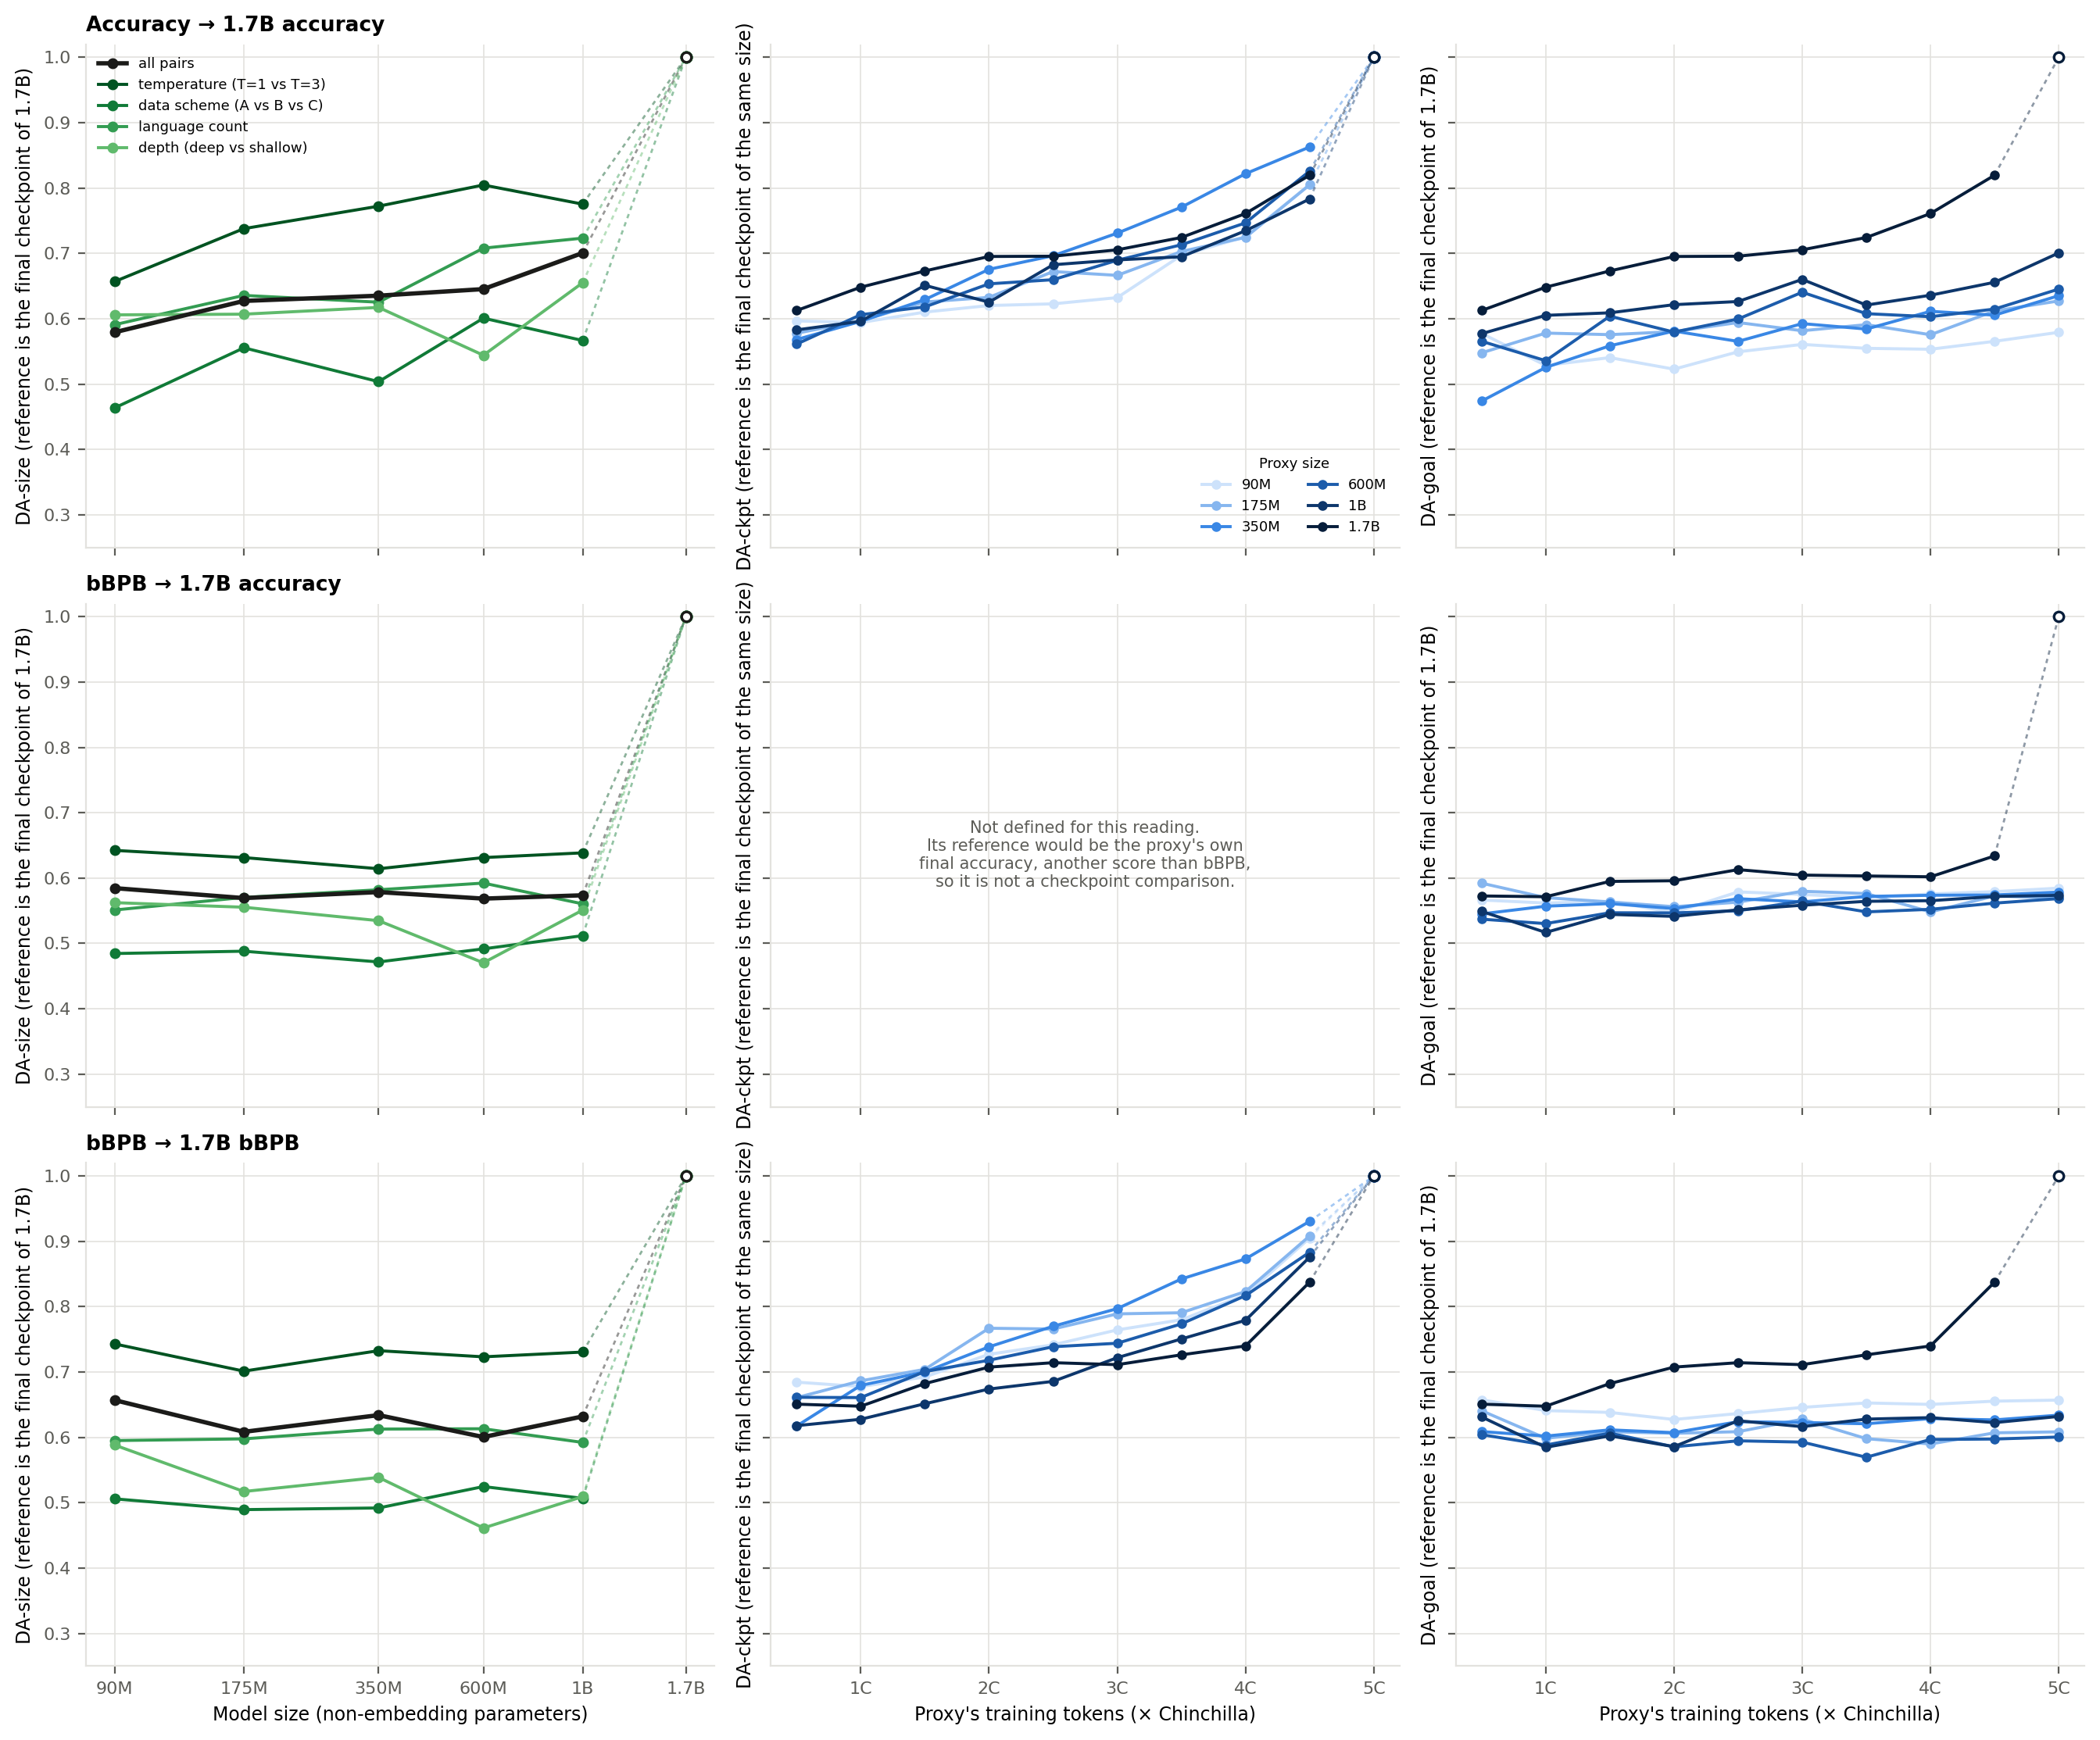
\includegraphics[width=\textwidth,height=0.8\textheight,keepaspectratio]{figures/app_rq02_bbpb.png}
% source: src/signal-and-noise/analysis/rq02_decision_accuracy/pretraining/predictivity/rq2_da_all_above_66_either_transformation_by_scoring_mono_axis.png
\caption{\textbf{Only accuracy decides more like the 1.7B reference as the proxy grows. The bBPB twins stay flat whichever 1.7B score they are ranked against.} This figure splits the panels of Figure~\ref{fig:rq2} by how a task is scored and what it is ranked against. Top row: accuracy (the original items and their RF and LLM-RF versions) against the 1.7B accuracy. Middle row: the bBPB twins, the bits per byte of the gold answer, against the 1.7B accuracy of their original task, kept where that accuracy is above chance at 1.7B. DA-ckpt is not defined there, since its reference would be the proxy's own final accuracy, a second score. Bottom row: all the twins against their own 1.7B bBPB, which has no chance level, so the gate keeps every twin. All rows use the mono-axis design pairs of the seed-1904 runs and the task filter of Figure~\ref{fig:rq2} (median DA-size or median DA-ckpt at least 0.66). DA-size over all pairs goes from 0.58 at 90M to 0.70 at 1B on accuracy over 85--121 tasks (the gate keeps more tasks at larger sizes). It stays at 0.57--0.58 for bBPB against accuracy over 410 tasks and at 0.60--0.66 for bBPB against bBPB over 621 tasks. Left: DA-size, one black line over all pairs and one green line per design axis. Middle: DA-ckpt. Right: DA-goal, one line per proxy size. A hollow point is 1.0 by comparing a ranking with itself.}
\label{fig:app_rq02_bbpb}
\end{figure*}
